\documentclass[border=5pt]{standalone}
\usepackage{amsmath}
\usepackage{tikz}
\usetikzlibrary{shapes}

\begin{document}

\begin{minipage}{15.5cm}
\begin{figure}[tb]
    \centering
\begin{tikzpicture}
\node[anchor=south west,inner sep=0] at (-3.31,-2.12) {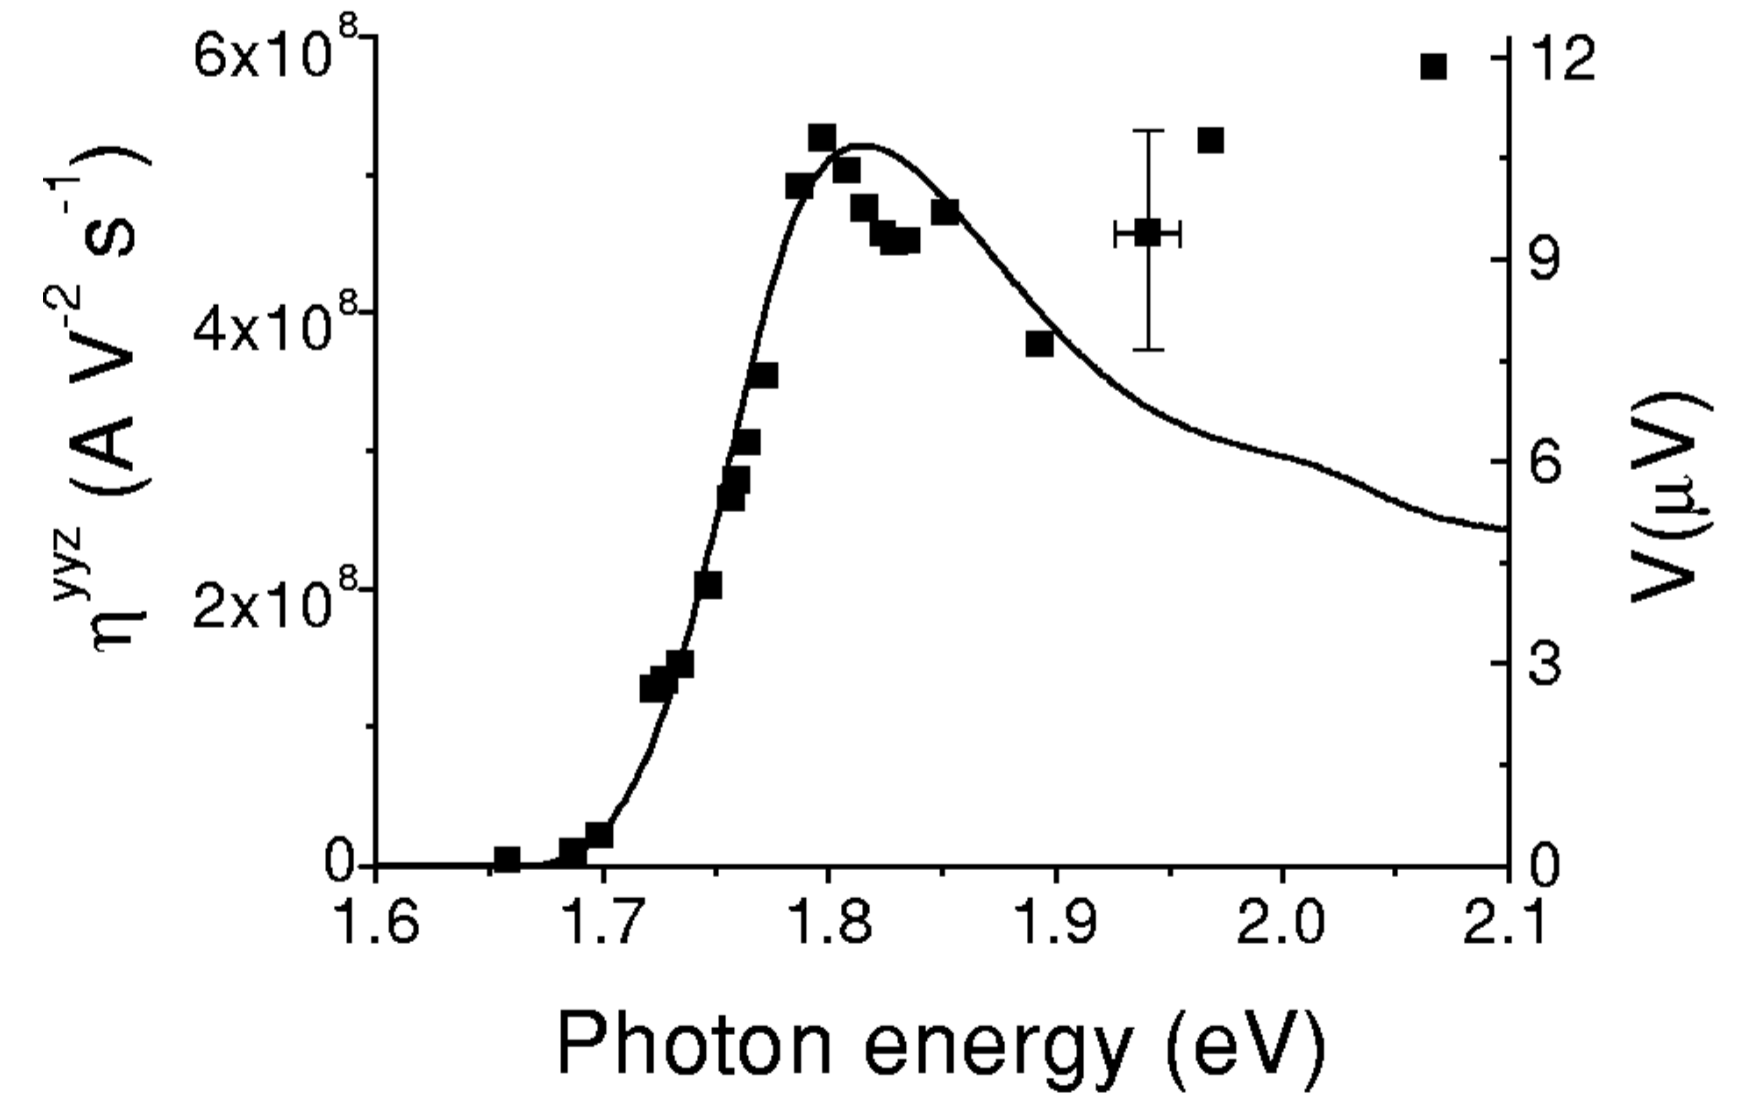
\includegraphics[width=15.35cm]{lamanAPL99-Fig3.png}};

% border:
    % border height: 
    \def \ymax {7.12}
    % border lenght
    \def \xmax {10.0}
    \draw[red, thick] (0,0) -- (\xmax,0) -- (\xmax,\ymax) -- (0,\ymax) -- cycle;

% subdivitions:
    % x and y divitions:
    \def \xdiv {10}
    \def \ydiv {12}
    \def \yDiv {\ydiv*10}

% grid:
    \def \ythickdiv {\ymax/\ydiv}
    \def \xthickdiv {\xmax/\xdiv}
    \def \ytindiv {\ydiv*10}
    % tin grid:
    \def \ytindiv {\ythickdiv*0.1}
    \foreach \i in {1,...,120}{\draw[green] (0,\ytindiv*\i) -- (\xmax,\ytindiv*\i);}
    \def \xtindiv {\xthickdiv*0.1}
    \foreach \i in {1,...,100}{\draw[green] (\xtindiv*\i,0) -- (\xtindiv*\i,\ymax);}
    % thick grid:
    \foreach \i in {1,...,\ydiv}{\draw[red, thick] (0,\ythickdiv*\i) -- (\xmax,\ythickdiv*\i);}
    \foreach \i in {1,...,10}{\draw[red, thick] (\xthickdiv*\i,0) -- (\xthickdiv*\i,\ymax);}

% experimental points:

\draw [blue, thick] (1.16,0) -- (1.16,7.3);
\draw [blue, thick] (1.74,0) -- (1.74,7.3);
\draw [blue, thick] (1.94,0) -- (1.94,7.3);
\draw [blue, thick] (2.44,0) -- (2.44,7.3);
\draw [blue, thick] (2.54,0) -- (2.54,7.3);
\draw [blue, thick] (2.70,0) -- (2.70,7.3);
\draw [blue, thick] (2.94,0) -- (2.94,7.3);
\draw [blue, thick] (3.14,0) -- (3.14,7.3);
\draw [blue, thick] (3.20,0) -- (3.20,7.3);
\draw [blue, thick] (3.30,0) -- (3.30,7.3);
\draw [blue, thick] (3.40,0) -- (3.40,7.3);
\draw [blue, thick] (3.74,0) -- (3.74,7.3);
\draw [blue, thick] (3.94,0) -- (3.94,7.3);
\draw [blue, thick] (4.14,0) -- (4.14,7.3);
\draw [blue, thick] (4.30,0) -- (4.30,7.3);
\draw [blue, thick] (4.50,0) -- (4.50,7.3);
\draw [blue, thick] (4.60,0) -- (4.60,7.3);
\draw [blue, thick] (4.70,0) -- (4.70,7.3);
\draw [blue, thick] (5.04,0) -- (5.04,7.3);
\draw [blue, thick] (5.86,0) -- (5.86,7.3);
\draw [blue, thick] (6.80,0) -- (6.80,7.3);
\draw [blue, thick] (7.34,0) -- (7.34,7.3);
\draw [blue, thick] (9.34,0) -- (9.34,7.3);
\end{tikzpicture}
\caption{Fig (3) from  APL \textbf{75}, 17 2581--2583 (1999). Original caption:
Calculated spectral dependence of  $\eta^{yyz}$ in CdSe. The data represent the
spectral dependence of current injection using a 130 fs optical paramet- ric
amplifier; the vertical scales have been chosen to yield a common peak
amplitude.}
\label{fig:experimental_data}
\end{figure}
Experimental data extracted:
\begin{center}
\begin{tabular}{ccc}
Point &   Photon energy (Ev) &  $V$ ($\mu$V)    \\    
01    &   1.658              &  0.15 \\
02    &   1.687              &  0.20 \\
03    &   1.697              &  0.45 \\
04    &   1.722              &  2.65 \\
05    &   1.727              &  2.80 \\
06    &   1.735              &  3.00 \\
07    &   1.747              &  4.20 \\
08    &   1.757              &  5.55 \\
09    &   1.760              &  5.75 \\
10    &   1.765              &  6.40 \\
11    &   1.770              &  7.40 \\
12    &   1.787              & 10.15 \\
13    &   1.797              & 10.80 \\
14    &   1.807              & 10.30 \\
15    &   1.815              &  9.80 \\
16    &   1.825              &  9.40 \\
17    &   1.830              &  9.30 \\
18    &   1.835              &  9.35 \\
19    &   1.852              &  9.70 \\
20    &   1.893              &  7.75 \\
21    &   1.940              &  9.20 \\
22    &   1.967              &  9.80 \\

23    &   2.067              & 11.85 \\

\end{tabular}
\end{center}

\end{minipage}


\end{document}



1.655    0.15
1.685    0.20
1.695    0.45
1.715    2.65
1.725    2.80
1.735    3.00
1.745    4.20
1.755    5.55
1.505    5.75
1.765    6.40
1.770    7.40
1.785   10.15
1.795   10.80
1.807   10.30
1.815    9.80
1.825    9.40
1.827    9.30
1.835    9.35
1.850    9.70
1.893    7.75
1.940    9.20
1.967    9.80
1.657   11.85
